\documentclass[11pt,a4paper]{article}
\usepackage[T1]{fontenc}
\usepackage[utf8]{inputenc}
\usepackage{amsfonts}
\usepackage{amssymb}
\usepackage{mdframed}
\usepackage{tikz}
\usepackage{tkz-tab}
\usepackage{pgfplots}
\usepgfplotslibrary{fillbetween}
\usepackage{xcolor}
\usepackage{fancyhdr}
\usepackage{lastpage}
\usepackage[fleqn]{amsmath}
\setlength{\mathindent}{0pt}

% Spécifications du document
\newcommand{\doctitre}{Les limites} % Ex: Le second degré
\newcommand{\docniveau}{T$^{\text{le}}$ Spécialité mathématiques} % Ex: ^{\text{re}}$ Spécialité mathématiques
\newcommand{\doctheme}{Analyse} %Ex: Algèbre
\newcommand{\doctype}{Démonstrations} % Ex: Démonstrations
\newcommand{\docshorttype}{Démo} % Démo

% Couleurs pour les graphiques
\definecolor{dark_green}{HTML}{008000}

% Paramètres du document
\RequirePackage{geometry}
\geometry{tmargin=1cm,bmargin=1.9cm,lmargin=1.9cm,rmargin=1.9cm}
\setlength{\parindent}{0pt}
\title{\doctitre}
\author{\docniveau \\ \doctheme\text{ - }\doctype}
\date{}
\fancypagestyle{custom}{
  \fancyhf{}
  \renewcommand{\headrulewidth}{0pt}
  \lfoot{\doctheme\text{ - }\docshorttype}
  \cfoot{\doctitre} % Change \titre to \doctitre
  \rfoot{\thepage/\pageref{LastPage}}
}

% Styles pour les mdframed
\mdfdefinestyle{definitionStyle}{
    leftline=true,
    rightline=false,
    topline=false,
    bottomline=false,
    linewidth=2pt,
    linecolor=black,
    innertopmargin=0pt,
    innerbottommargin=0pt,
    innerrightmargin=0pt,
    innerleftmargin=5pt,
}

\mdfdefinestyle{proprieteStyle}{
    linewidth=1pt,
    linecolor=black,
    innertopmargin=5pt,
    innerbottommargin=5pt,
    innerrightmargin=5pt,
    innerleftmargin=5pt,
}
% ----- DEBUT DU DOCUMENT -----
\begin{document}

% Style et numérotation
\maketitle
\pagestyle{custom}
\thispagestyle{custom}

\section{Limites finies d'une fonction en $+\infty$}

\textbf{Démonstration du Théorème 1 :} ~\\

\begin{minipage}{0.5\textwidth}
    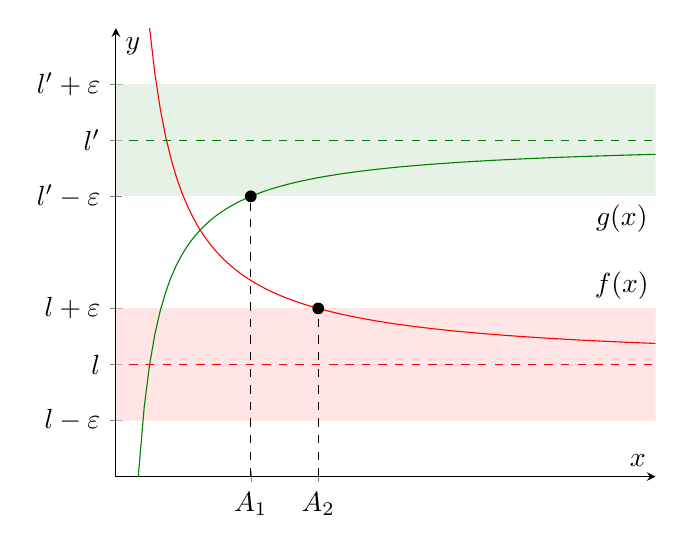
\begin{tikzpicture}
        \begin{axis}[
            axis lines=middle,
            xlabel={$x$},
            ylabel={$y$},
            xtick={2, 3},
            xticklabels={$A_1$, $A_2$},
            ytick={0.5, 1, 1.5, 2.5, 3, 3.5},
            yticklabels={$l-\varepsilon$, $l$, $l+\varepsilon$, $l'-\varepsilon$, $l'$, $l'+\varepsilon$},
            xmin=0, xmax=8,
            ymin=0, ymax=4,
            samples=100
        ]
        \addplot[red, domain=0.1:8] {1.5/x + 1};
        \addplot[dark_green, domain=0.1:8] {-1/x + 3};
        \addplot[dashed, red, domain=0.2:8] {1};
        \addplot[dashed, dark_green, domain=0.2:8] {3};
    
        % Define the vertical lines for intervals
        \path[name path=axis] (axis cs:0,0) -- (axis cs:8,0);
        \path[name path=line1] (axis cs:0,1.5) -- (axis cs:8,1.5);
        \path[name path=line2] (axis cs:0,0.5) -- (axis cs:8,0.5);
        \path[name path=line3] (axis cs:0,2.5) -- (axis cs:8,2.5);
        \path[name path=line4] (axis cs:0,3.5) -- (axis cs:8,3.5);
    
        % Fill between the paths
        \addplot[fill=red!20, fill opacity=0.5] fill between[of=line1 and line2];
        \addplot[fill=dark_green!20, fill opacity=0.5] fill between[of=line3 and line4];
        
        % Add function names
        \node at (axis cs:7.5, 1.7) {$f(x)$};
        \node at (axis cs:7.5, 2.3) {$g(x)$};
    
        % Add points
        \node[circle,fill,inner sep=1.5pt] at (axis cs:3,1.5) {};
        \node[circle,fill,inner sep=1.5pt] at (axis cs:2,2.5) {};
    
        % Add lines
        \addplot[dashed] coordinates {(3, 0) (3, 1.5)};
        \addplot[dashed] coordinates {(2, 0) (2, 2.5)};
    
    
        \end{axis}
    
    \end{tikzpicture}

\end{minipage}
\hfill
\begin{minipage}{0.5\textwidth}
    

    On choisit $\varepsilon$ tel que $l+\varepsilon < l'-\varepsilon$. 

    En supposant que $f$ tend vers $l$ : il existe $A_1$ tel que pour tout $x>A_1$ : $l-\varepsilon < f(x) < l+\varepsilon$.
    
    En supposant que $g$ tend vers $l'$ : il existe $A_2$ tel que pour tout $x>A_2$ : $l'-\varepsilon < g(x) < l'+\varepsilon$.
    
    En prenant $A=\max(A_1, A_2)$, pour tout $x>A$ on a :
    \begin{itemize}
        \item $x>A_1$ donc $f(x)<l+\varepsilon$
        \item $x>A_2$ donc $g(x)>l'-\varepsilon$
    \end{itemize}
    
    Donc $f(x)< l+\varepsilon < l'-\varepsilon < g(x)$ donc $f(x)<g(x)$.
\end{minipage}

\text{ }\\

\textbf{Démonstration du Théorème 2 :} ~\\

Par l'absurde, supposons que $l>l'$ et $\displaystyle\lim_{x \to +\infty} f(x) = l$ et $\displaystyle\lim_{x \to +\infty} g(x) = l'$
et il existe $A$ réel tel que pour tout $x>A$ : $f(x)\leq g(x)$.

D'après le Théorème 1, sous les hypothèses ci-dessus, il existe un réel $A'$ tel que pour tout $x>A'$, $f(x)>g(x)$.

Ceci entre en contradiction avec la 4$^e$ hypothèse ($f(x)\leq g(x)$). Conclusion : $l<l'$.

\end{document}
% ----- FIN DU DOCUMENT -----